% !TEX root = ../om_ts_01.tex

\begin{frame} % название фрагмента

\videotitle{Характеристики рядов}

\end{frame}



\begin{frame}{Характеристики рядов: план}
  \begin{itemize}[<+->]
    \item Выборочная автокорреляция. 
    \item Выборочная частная автокорреляция.
    \item STL-характеристики.
  \end{itemize}

\end{frame}

\begin{frame}{Задачи для множества рядов}
  \begin{itemize}
    \item Классифицировать новый ряд в один из существующих классов.
    \item Понять, какие ряды близки к друг другу.
    \item Кластеризовать ряды на неизвестное множество кластеров.
  \end{itemize}
  \pause
  \alert{Как решить?}
  \begin{enumerate}[<+->]
    \item Для каждого ряда сгенерировать \alert{признаки}. 
    \item К полученным признакам применить алгоритм для перекрестных данных.
 \end{enumerate}
 \pause
 Классифицировать: с помощью случайного леса.

 Измерить расстояние с помощью метрики Махаланобиса. 

 Кластеризовать с помощью иерархической кластеризации. 

\end{frame}


\begin{frame}{Создаём признаки}

Два \alert{множества} признаков:
\begin{itemize}[<+->]
  \item Выборочная ACF (\alert{автокорреляционная функция}, AutoCorrelation Function).
  \item Выборочная PACF (\alert{частная} автокорреляционная функция, Partial ACF).
\end{itemize}

\pause
Из \alert{одного} ряд получим:

$ACF_1$, $ACF_2$, $ACF_3$, \ldots

$PACF_1$, $PACF_2$, $PACF_3$, \ldots
\end{frame}


\begin{frame}{ACF}

\begin{block}{Выборочная ACF}
  Оценим множество парных регрессий:
  \[
  \hat y_t = \hat\beta_1 + \hat\beta_2 y_{t-1}, \quad ACF_1 = \hat\beta_2;
  \]
  \pause
  \[
    \hat y_t = \hat\beta_1 + \hat\beta_2 y_{t-2}, \quad ACF_2 = \hat\beta_2;
  \]
  \pause
  \[
    \hat y_t = \hat\beta_1 + \hat\beta_2 y_{t-k}, \quad ACF_k = \hat\beta_2;
  \]
\end{block}

\pause
\alert{Смысл}
$ACF_2$: на сколько единиц в среднем $y_t$ выше среднего, если $y_{t-2}$ выше среднего на одну единицу.

\end{frame}


\begin{frame}{Ряд и его ACF}

  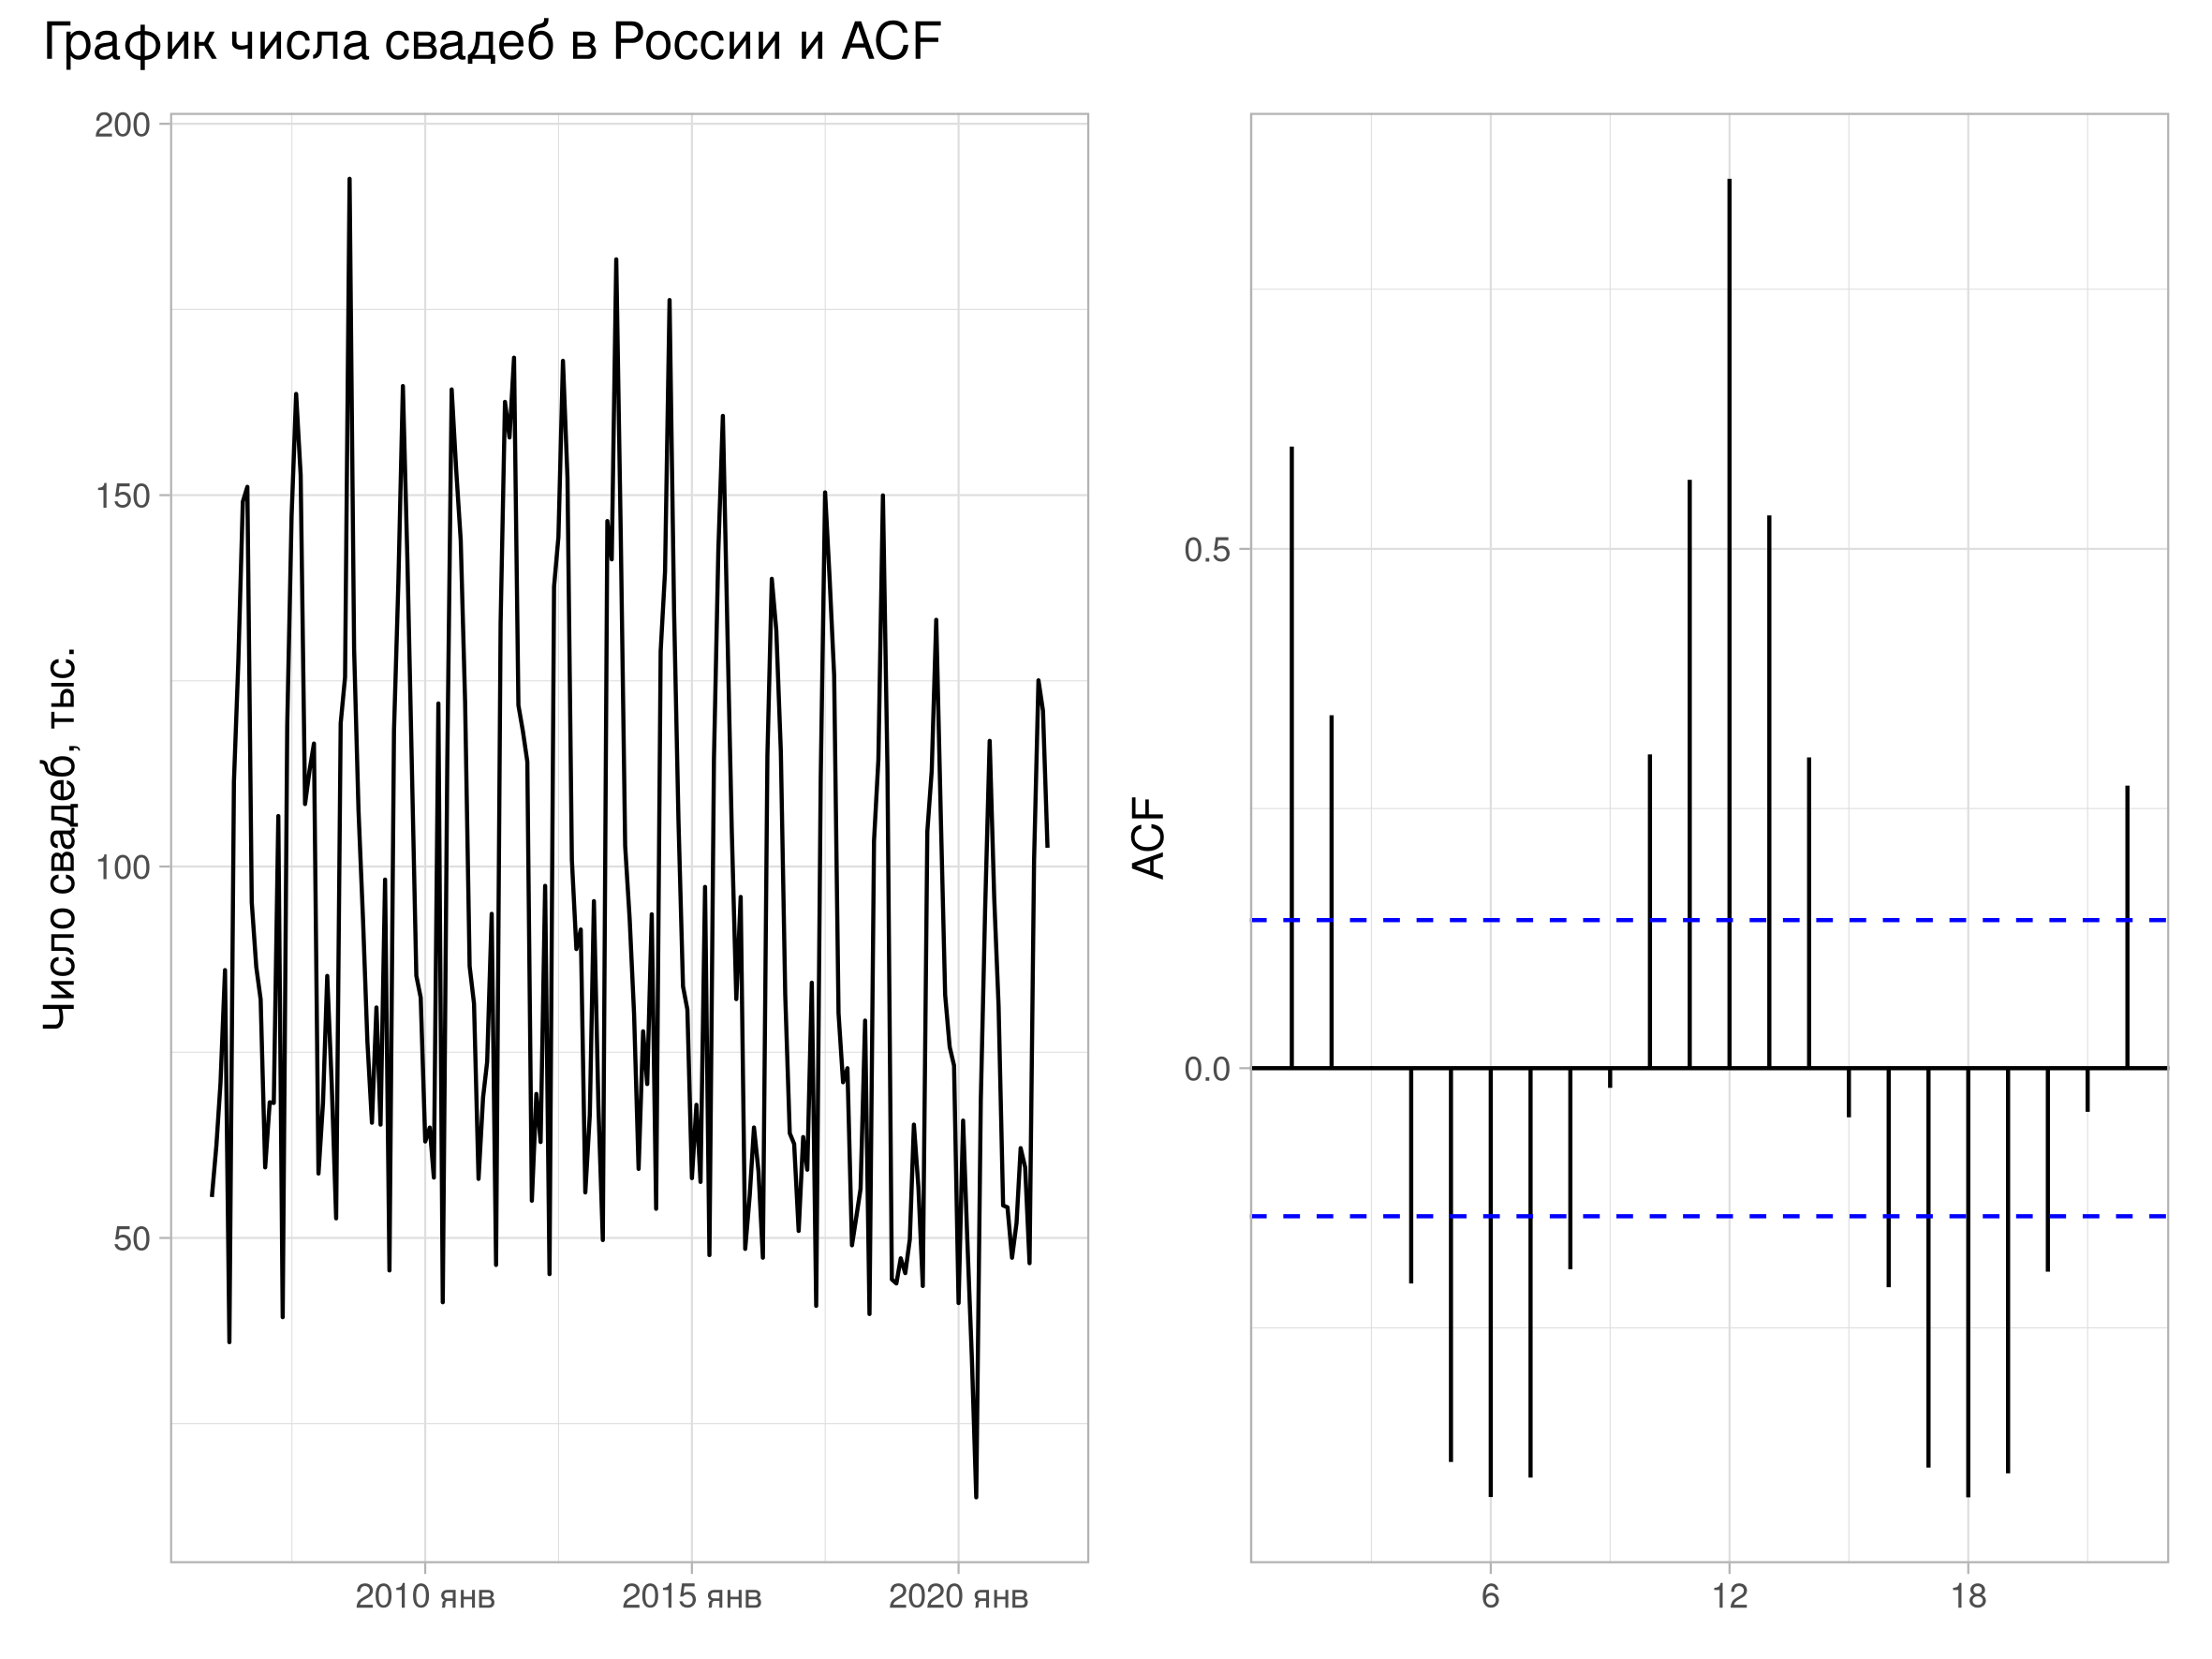
\includegraphics[width=\textwidth]{pictures/om_ts_01-120.png}

\end{frame}

\begin{frame}{Почему ACF — корреляция?}

  \alert{Классическое определение}

  \begin{block}{Выборочная ACF}
    $ACF_k$ — выборочная корреляция между рядом $y_t$ и рядом $y_{t-k}$.
  \end{block}

\pause
Различие между определениями \alert{мало}. 

\end{frame}


\begin{frame}{PACF}

  \begin{block}{Выборочная PACF}
    Оценим множество множественных регрессий:
    \[
    \hat y_t = \hat\alpha + \hat\beta_1 y_{t-1}, \quad PACF_1 = \hat\beta_1;
    \]
    \pause
    \[
      \hat y_t = \hat\alpha  + \hat\beta_1 y_{t-1} + \hat\beta_2 y_{t-2}, \quad PACF_2 = \hat\beta_2;
    \]
    \pause
    \[
      \hat y_t = \hat\alpha + \hat\beta_1 y_{t-1} + \ldots + \hat\beta_k y_{t-k}, \quad PACF_k = \hat\beta_k;
    \]
  \end{block}
  
  \pause
  \alert{Смысл}
  $PACF_2$: на сколько единиц в среднем $y_t$ выше среднего, если $y_{t-2}$ выше среднего на одну единицу,
  а $y_{t-1}$ на среднем уровне.

  \end{frame}
  
  \begin{frame}{Ряд и его PACF}

    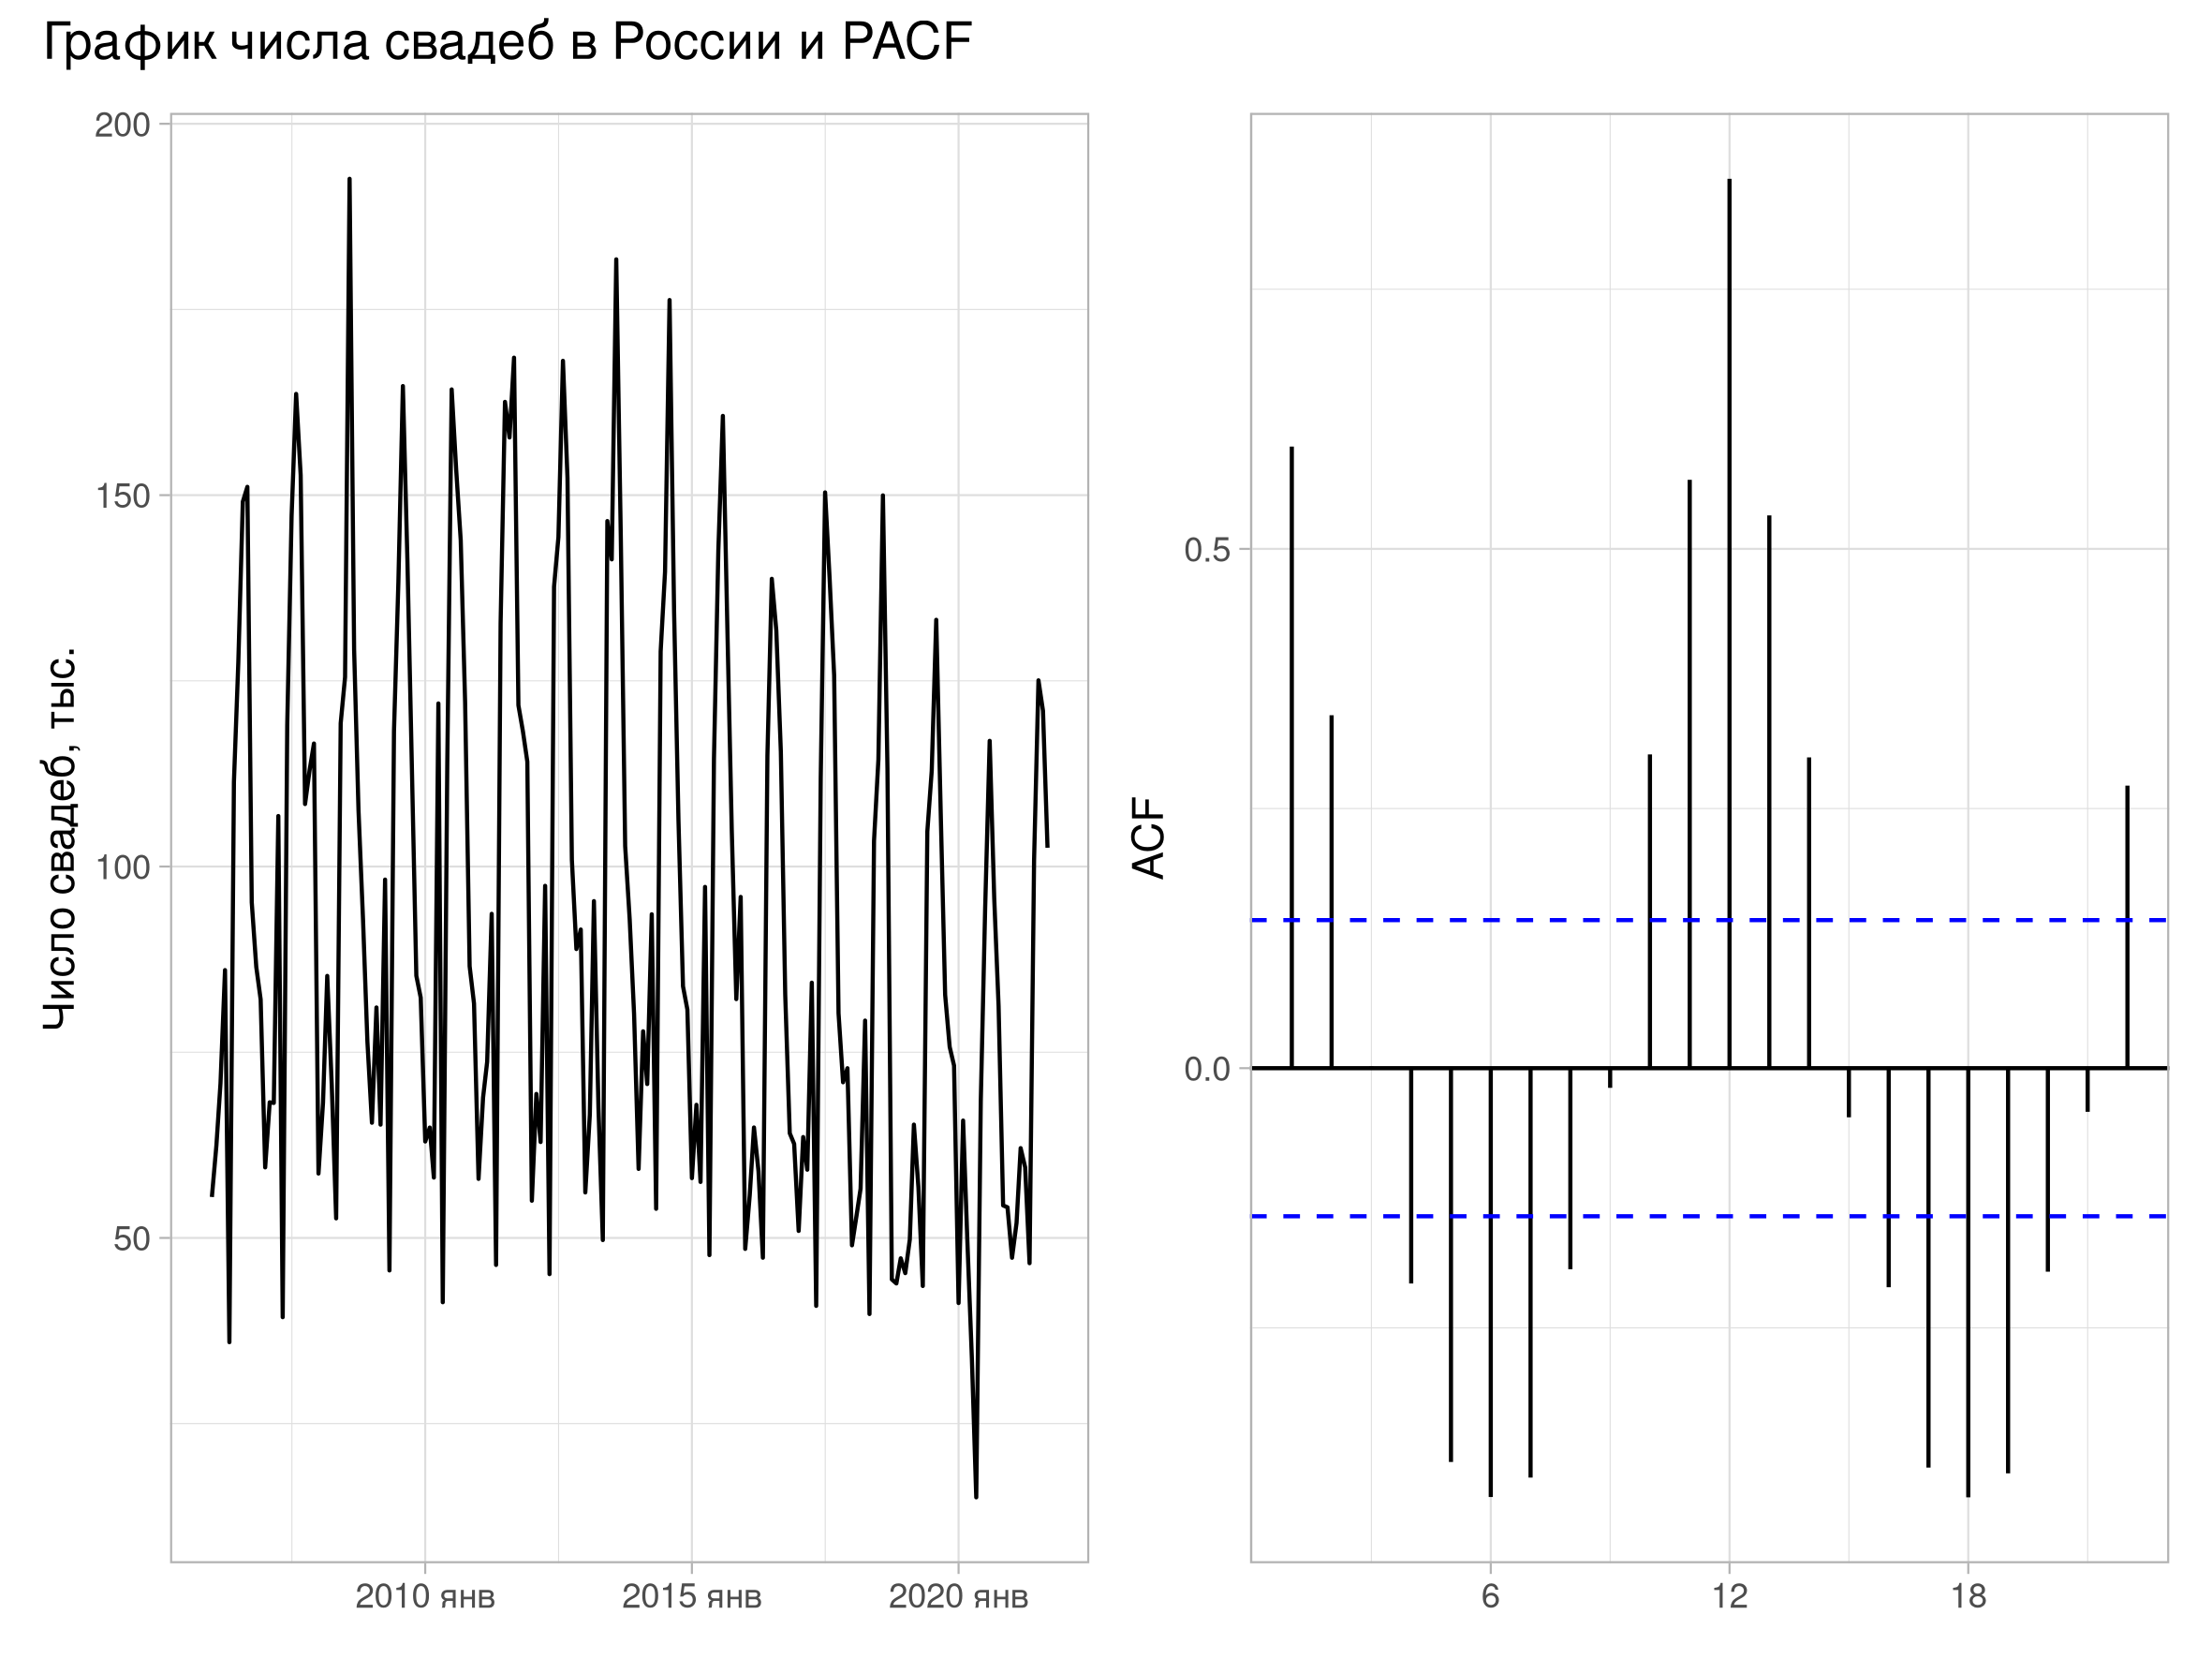
\includegraphics[width=\textwidth]{pictures/om_ts_01-127.png}
    
  \end{frame}
    
  \begin{frame}{Почему PACF — корреляция?}

    \alert{Классическое определение}
  
    \begin{block}{Выборочная PACF}
      $PACF_4$ — выборочная корреляция между остатками $a_t$ и остатками $b_t$.

      $a_t$ — остатки из регрессии
      \[
        y_t \text{ на } 1, y_{t-1}, y_{t-2}, y_{t-3}.
      \]

      $b_t$ — остатки из регрессии
      \[
        y_{t-4} \text{ на } 1, y_{t-1}, y_{t-2}, y_{t-3}.
      \]
    \end{block}
  
  \pause
  Различие между определениями \alert{мало}. 
  
  \end{frame}
  

  \begin{frame}{STL-характеристики}

    \alert{На выходе:}
    \[
      y_t = T_t + S_t + R_t.
    \]

    \pause
    Измерим:
    \begin{itemize}
      \item Выраженность тренда $F_{trend}$.
      \item Выраженность сезонности $F_{seas}$.
    \end{itemize}

  \end{frame}

  \begin{frame}{Выраженность тренда и сезонности}

    Получили разложение:
    \[
      y_t = trend_t + seas_t + remainder_t.
    \]
    
    \pause
    \alert{Идея определения:}
    При идеальном разложении с некоррелированными компонентами:
    \[
      F_{trend} = \frac{\sVar(trend)}{\sVar(trend) + \sVar(remainder)},
    \]

    \pause
    \[
    F_{seas} = \frac{\sVar(seas)}{\sVar(seas) + \sVar(remainder)},
  \]
  \end{frame}

  \begin{frame}{Выраженность тренда и сезонности}

    Получили разложение:
    \[
      y_t = trend_t + seas_t + remainder_t.
    \]

    \pause
    \alert{На практике}:
    \begin{itemize}[<+->]
      \item Выраженность тренда:
      \[
        F_{trend} = \max\left\{1 - \frac{\sVar(remainder)}{\sVar(trend + remainder)}, 0 \right\}.
      \]
      \item Выраженность сезонности:
      \[
        F_{seas} = \max\left\{1 - \frac{\sVar(remainder)}{\sVar(seas + remainder)}, 0 \right\}.
      \]

    \end{itemize}



  \end{frame}


  \begin{frame}{Выраженность тренда и сезонности}

    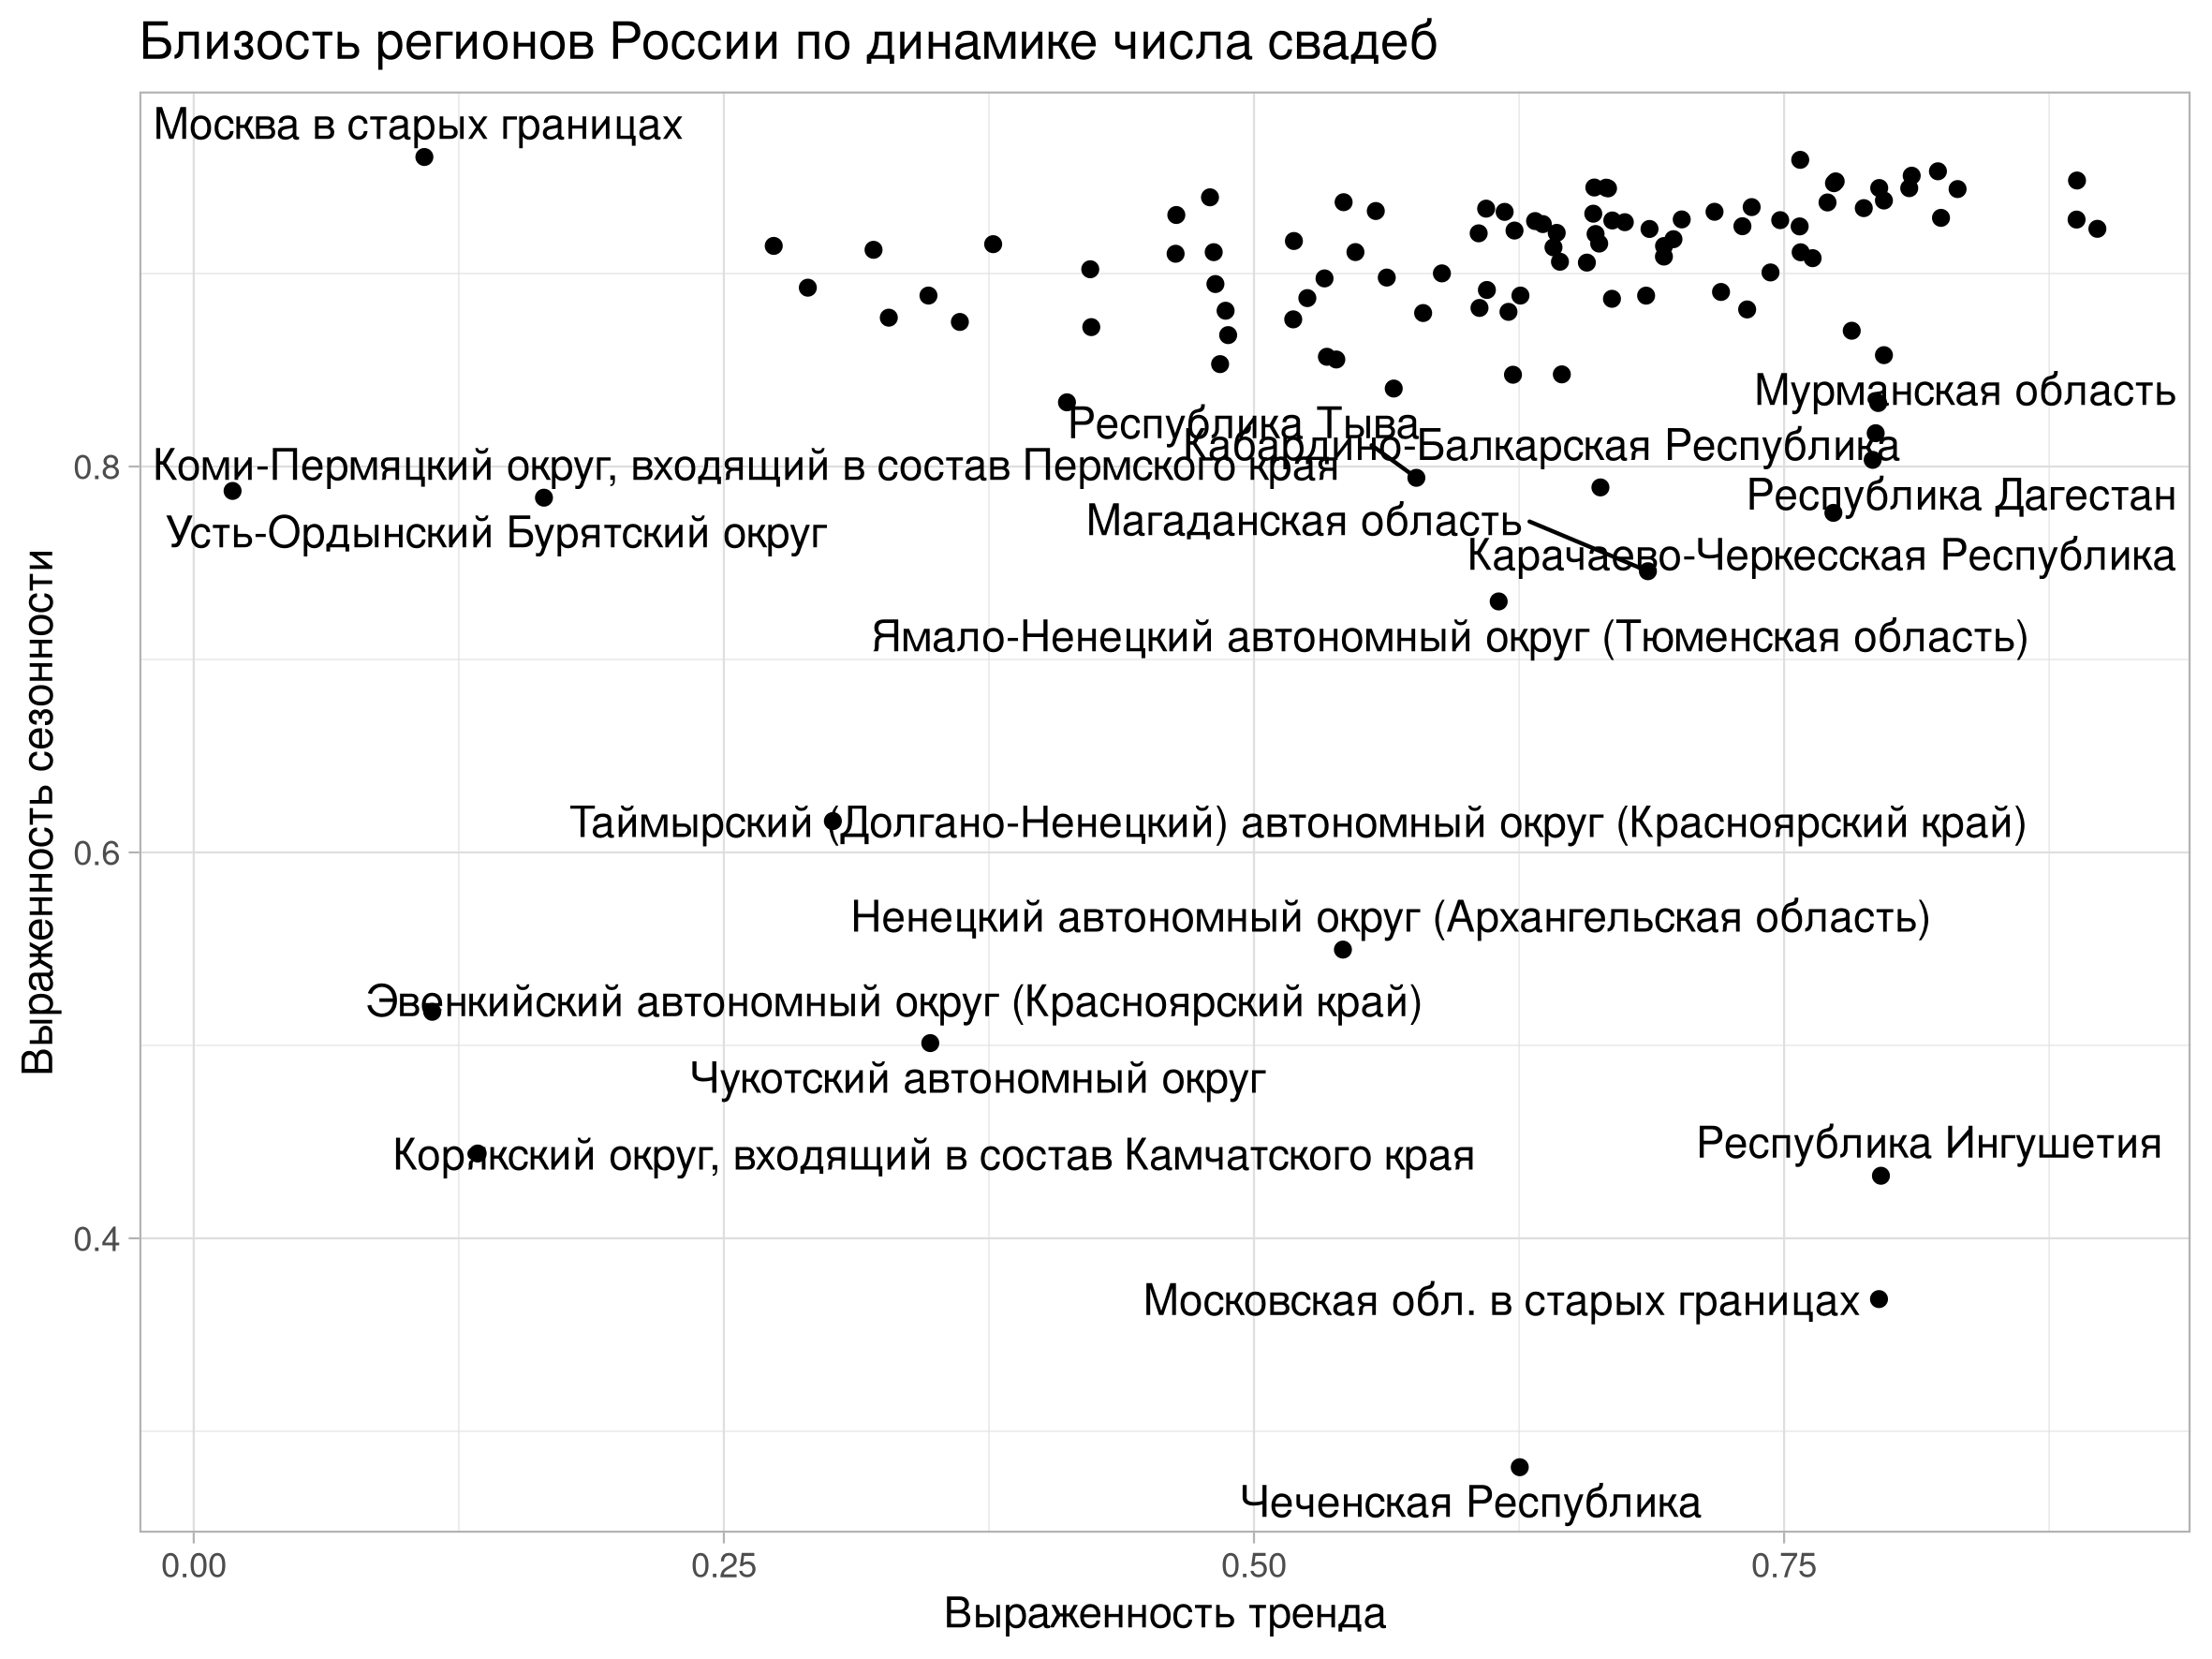
\includegraphics[width=\textwidth]{pictures/om_ts_01-138.png}

    
  \end{frame}
  


\begin{frame}{Характеристики рядов: итоги}

  \begin{itemize}[<+->]
    \item ACF — коэффициенты в \alert{парных} регрессиях или корреляции.
    \item PACF — коэффициенты во \alert{множественных} регрессиях или корреляции.
    \item STL позволяет измерить \alert{выраженность тренда и сезонности} по сравнению с остаточной компонентой.
  \end{itemize}
\end{frame}

